\documentclass [11pt]{article}

\usepackage{amsmath}
\usepackage{amsfonts}
\usepackage{amssymb}
\usepackage{graphicx}
\usepackage{subcaption}
\usepackage{float}
\usepackage{fancyvrb}


\title{INF4490 Mandatory Assignment 1: \\ Travelling Salesman Problem}
\author{Minh Chien Nguyen (davidngcz@gmail.com)}

\begin{document}
\maketitle
\nocite{*}

\section{Introduction}
dfgagf\\
\\
faf
\section{Results}
\subsection{Franke}
\begin{figure}[H]
\centering
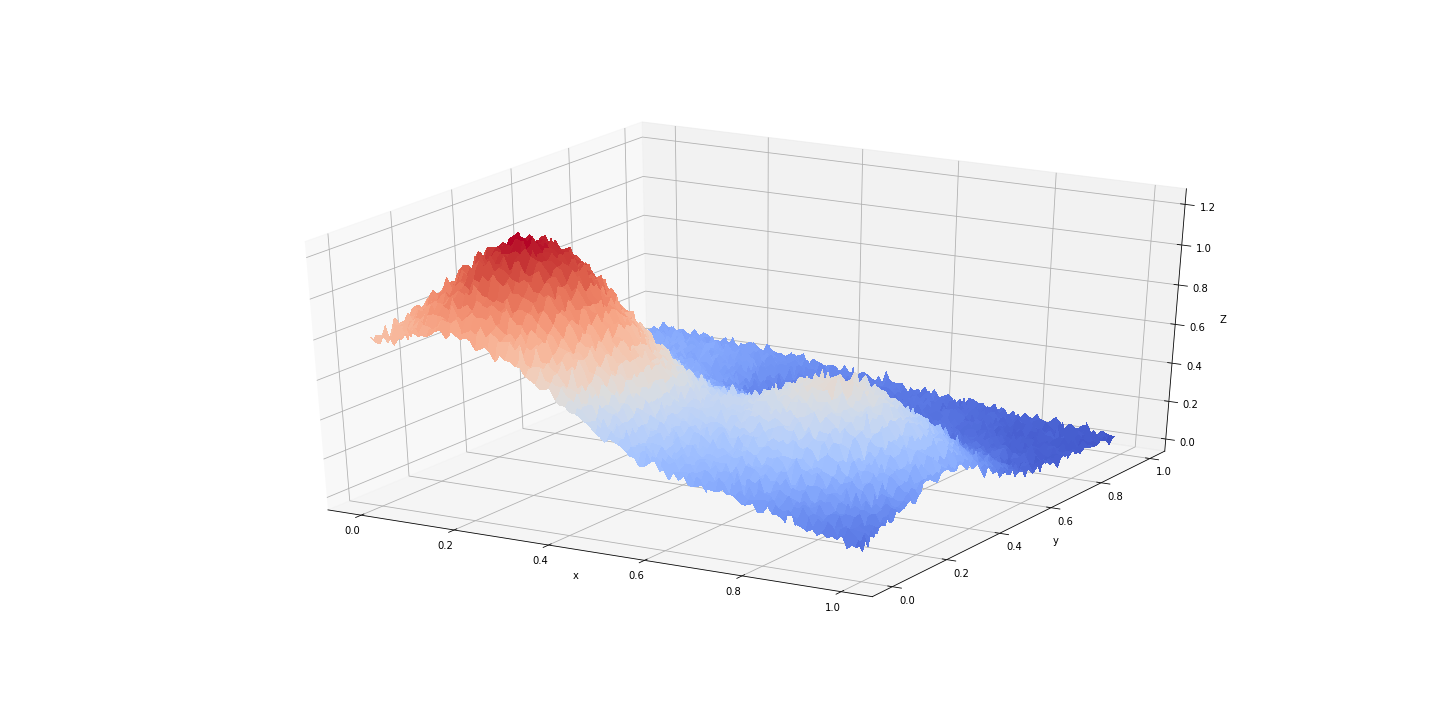
\includegraphics[width=1\textwidth]{figures/Franke.png}
        \caption{Average fitness of the best fit individual in each generation for $24$ cities using Baldwinian GA}
        \label{fig:Franke}
\end{figure}
\subsubsection{OLS}
efsdfs

\begin{table}[H]
\centering
%\resizebox{\textwidth}{!}{%
\begin{tabular}{lll}
\hline
  & MSE    & R2 score \\ \hline
3 & 0.0082 & 0.9      \\
4 & 0.0044 & 0.94     \\
5 & 0.0025 & 0.97     \\ \hline
\end{tabular}%
%}
\caption{My caption}
\label{my-label}
\end{table}

\begin{figure}[H]
\centering
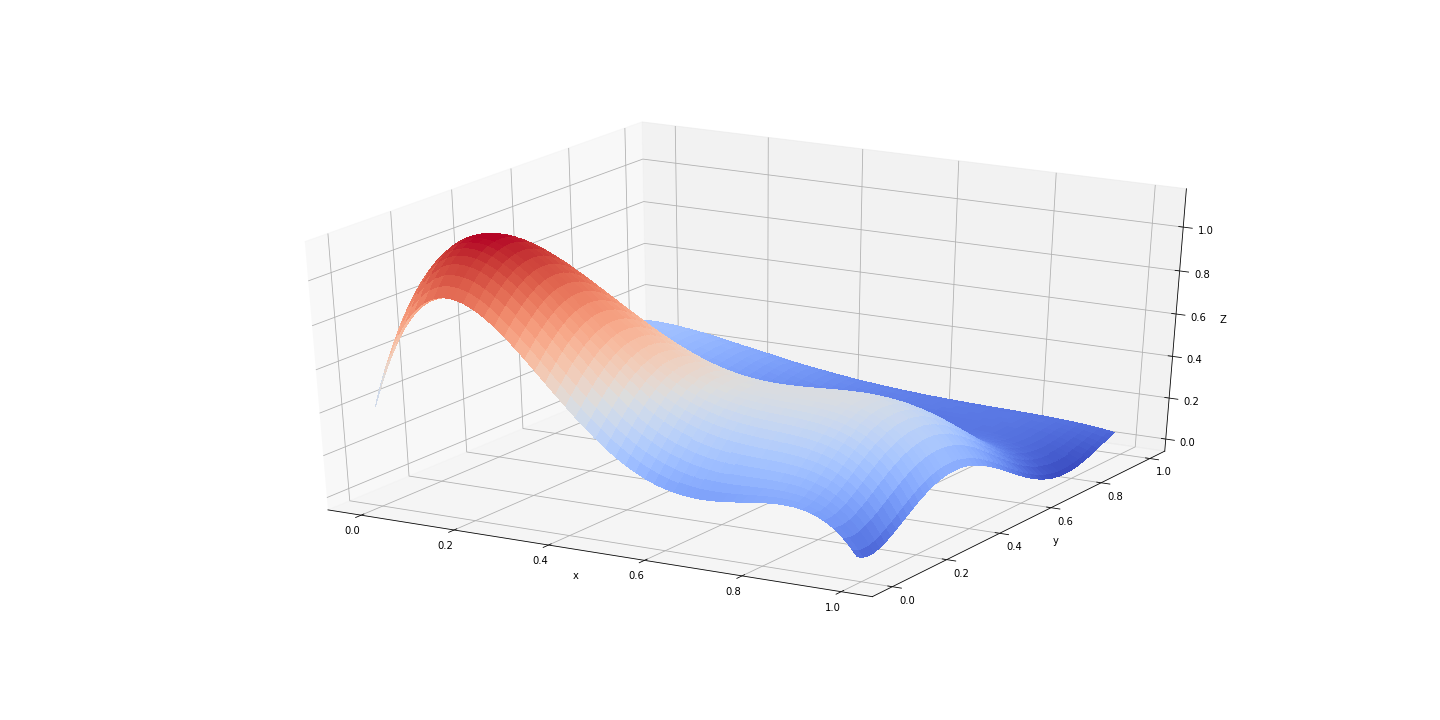
\includegraphics[width=1\textwidth]{figures/olsFranke.png}
        \caption{Average fitness of the best fit individual in each generation for $24$ cities using Baldwinian GA}
        \label{fig:olsFranke}
\end{figure}
Bias for the final model is: 24.627991661784236
Var for the final model is: 6.718071568281006e-07
\subsubsection{Ridge}

\begin{table}[H]
\centering
\begin{tabular}{lll}
\hline
$\lambda$ & MSE    & $R^{2}$ score \\ \hline
0.001     & 0.0082 & 0.90          \\
0.01      & 0.0082 & 0.90          \\
0.1       & 0.0082 & 0.90          \\
1         & 0.0102 & 0.87          \\
10        & 0.0161 & 0.80          \\
100       & 0.0235 & 0.71          \\ \hline
\end{tabular}
\caption{order3}
\label{my-label}
\end{table}

\begin{table}[H]
\centering
\begin{tabular}{lll}
\hline
$\lambda$ & MSE    & $R^{2}$ score \\ \hline
0.001     & 0.0043 & 0.94          \\
0.01      & 0.0047 & 0.94          \\
0.1       & 0.0071 & 0.91          \\
1         & 0.0091 & 0.88          \\
10        & 0.0137 & 0.83          \\
100       & 0.0223 & 0.73          \\ \hline
\end{tabular}
\caption{order 4}
\label{my-label}
\end{table}

\begin{table}[H]
\centering
\begin{tabular}{lll}
\hline
$\lambda$ & MSE    & $R^{2}$ score \\ \hline
0.001     & 0.0027 & 0.96          \\
0.01      & 0.0037 & 0.95          \\
0.1       & 0.0056 & 0.93          \\
1         & 0.0089 & 0.89          \\
10        & 0.0124 & 0.85          \\
100       & 0.0213 & 0.74          \\ \hline
\end{tabular}
\caption{order 5}
\label{my-label}
\end{table}

\begin{figure}[H]
\centering
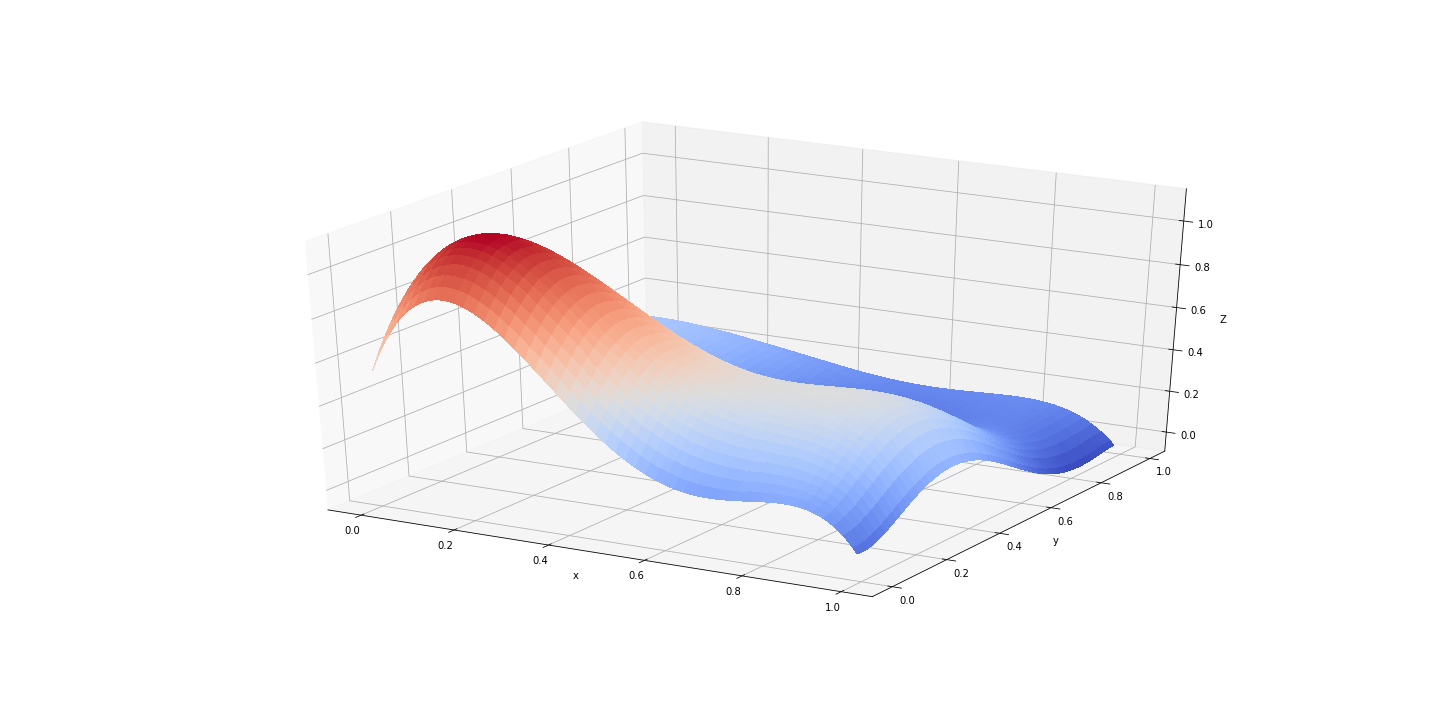
\includegraphics[width=1\textwidth]{figures/RidgeFranke.png}
        \caption{Average fitness of the best fit individual in each generation for $24$ cities using Baldwinian GA}
        \label{fig:RidgeFranke}
\end{figure}

Bias for the final model is: 26.93124204070874
Var for the final model is: 4.790683011567965e-07
\subsubsection{Lasso}

\begin{table}[H]
\centering
\begin{tabular}{lll}
\hline
$\lambda$ & MSE    & $R^{2}$ score \\ \hline
0.001     & 0.0180 & 0.78          \\
0.01      & 0.0254 & 0.69          \\
0.1       & 0.0830 & -0.0011       \\
1         & 0.0830 & -0.0011       \\
10        & 0.0830 & -0.0011       \\
100       & 0.0830 & -0.0011       \\ \hline
\end{tabular}
\caption{3}
\label{my-label}
\end{table}

\begin{table}[]
\centering
\begin{tabular}{lll}
\hline
$\lambda$ & MSE    & $R^{2}$ score \\ \hline
0.001     & 0.0142 & 0.82          \\
0.01      & 0.0254 & 0.69          \\
0.1       & 0.0830 & -0.0011       \\
1         & 0.0830 & -0.0011       \\
10        & 0.0830 & -0.0011       \\
100       & 0.0830 & -0.0011       \\ \hline
\end{tabular}
\caption{4}
\label{my-label}
\end{table}

\begin{table}[]
\centering
\begin{tabular}{lll}
\hline
$\lambda$ & MSE    & $R^{2}$ score \\ \hline
0.001     & 0.0135 & 0.83          \\
0.01      & 0.0254 & 0.69          \\
0.1       & 0.0830 & -0.0011       \\
1         & 0.0830 & -0.0011       \\
10        & 0.0830 & -0.0011       \\
100       & 0.0830 & -0.0011       \\ \hline
\end{tabular}
\caption{5}
\label{my-label}
\end{table}

\begin{figure}[H]
\centering
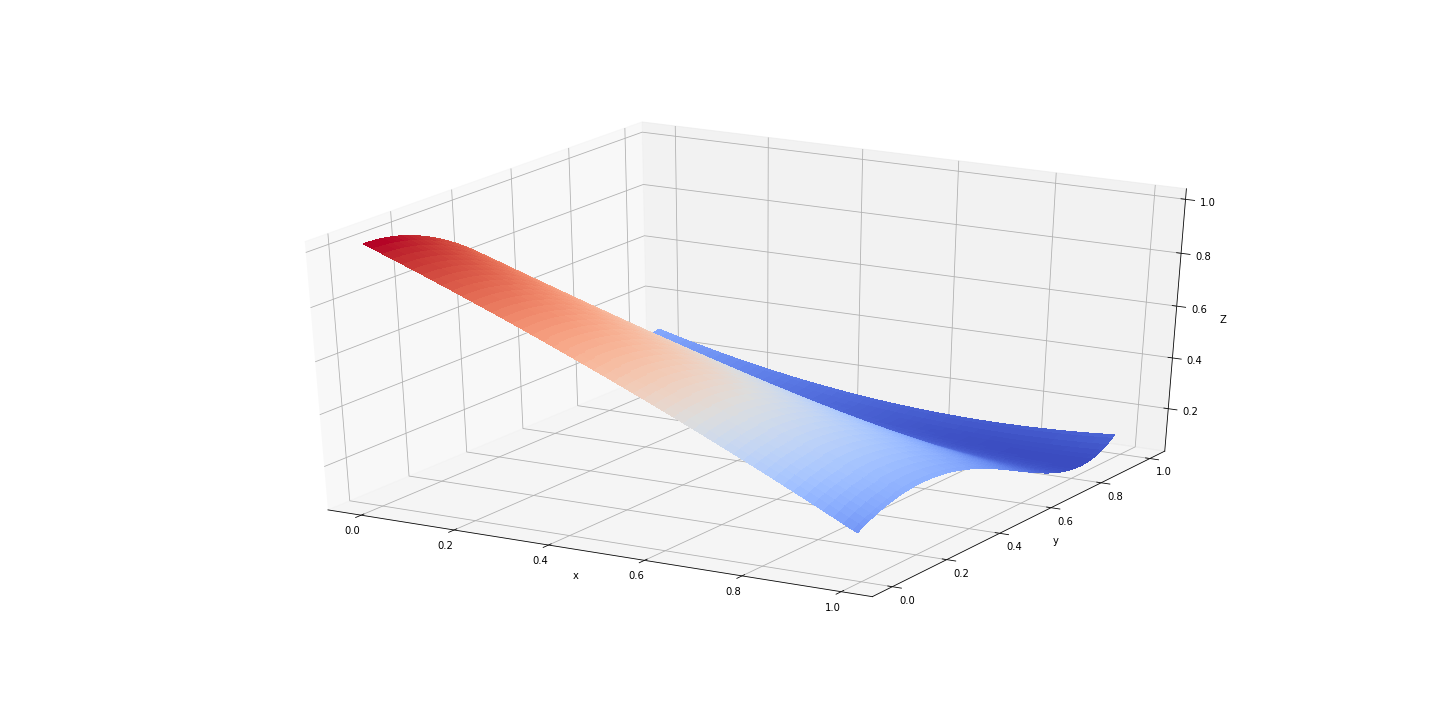
\includegraphics[width=1\textwidth]{figures/LassoFranke.png}
        \caption{Average fitness of the best fit individual in each generation for $24$ cities using Baldwinian GA}
        \label{fig:LassoFranke}
\end{figure}

Bias for the final model is: 134.818068147102
Var for the final model is: 1.0388557141474813e-06
\begin{thebibliography}{111}
\raggedright
\bibitem{abc} EIBEN, Agoston E., et al. Introduction to evolutionary computing. Berlin: springer, 2003.
\bibitem{def} MARSLAND, Stephen. Machine learning: an algorithmic perspective. Chapman and Hall/CRC, 2011.

\end{thebibliography}
\end{document}